\documentclass[a4paper,11pt]{article}
\usepackage[verbose,a4paper,tmargin=2cm,bmargin=2cm,lmargin=2.5cm,rmargin=2.5cm]{geometry}
\usepackage[utf8]{inputenc}
\usepackage{polski}
\usepackage{amsmath}
\usepackage{amsfonts}
\usepackage{amssymb}
\usepackage{lastpage}
\usepackage{indentfirst}
\usepackage{verbatim}
\usepackage{graphicx}
\usepackage{fancyhdr}
\usepackage{listings}
\usepackage{hyperref} 
\usepackage{xcolor}
\usepackage{tikz}

\usepackage{array,multirow,graphicx}
\usepackage{float}

\frenchspacing
\pagestyle{fancyplain}
\fancyhf{}
\renewcommand{\headrulewidth}{0pt}
\renewcommand{\footrulewidth}{0.4pt}
\newcommand{\degree}{\ensuremath{^{\circ}}} 
\fancyfoot[L]{MI: Justyna Hubert 210200, Karol Podlewski 210294}
\fancyfoot[R]{\thepage\ / \pageref{LastPage}}


\begin{document}

\begin{titlepage}
\begin{center}
\begin{tabular}{rl}
\begin{tabular}{|r|}
\hline \\
\large{\underline{210200~~~~~~~~~~~~~~~~~~~~~~~~~~~~~~~~~~~~~~~~~~} }\\
$^{numer\ indeksu}$\\
\large {\underline{Justyna Hubert~~~~~~~~~~~~~~~~~~~~~~~~~~~~~~} }\\
$^{imie\ i\ nazwisko}$ \\\\ \hline
\end{tabular} 
&
\begin{tabular}{|r|}
\hline \\
\large{\underline{210294~~~~~~~~~~~~~~~~~~~~~~~~~~~~~~~~~~~~~~~~~~} }\\
$^{numer\ indeksu}$\\
\large {\underline{Karol Podlewski~~~~~~~~~~~~~~~~~~~~~~~~~~~~~~} }\\
$^{imie\ i\ nazwisko}$ \\\\ \hline
\end{tabular} 

\end{tabular}
~\\~\\~\\ 
\end{center}
\begin{tabular}{ll}
\LARGE{\textbf{Data}}& \LARGE{20.10.2019}\\
\LARGE{\textbf{Kierunek}}& \LARGE{Informatyka}\\
\LARGE{\textbf{Rok akademicki}}& \LARGE{2019/20} \\
\LARGE{\textbf{Semestr}}& \LARGE{7} \\
\LARGE{\textbf{Specjalizacja}}& \LARGE{IOAD} \\
\LARGE{\textbf{Grupa dziekańska}}& \LARGE{3} \\~\\~\\~\\~\\
\end{tabular}

\begin{center}
\textbf{\Huge{\\~\\Marketing Internetowy\\~\\~\\~\\~\\}}
\end{center}


\begin{center}
\textbf{\Large{Zadanie 1\\Analiza i ocena wybranych witryn internetowych}}
\textbf{\Huge{\\~\\Wydawnictwa Gier Fabularnych}}	
\end{center}

\end{titlepage}
\setcounter{page}{2}


\section {Charakterystyka branży}

Gry fabularne są względnie nowym, dopiero rozwijającym się rynkiem wydawniczym. Pierwszy tytuł, wydany za oceanem, pojawił się w komercyjnej dystrybucji w roku 1974, a było to Dungeons \& Dragons wydane ówcześnie przez TSR. Branża ta od początku była niszową, by nie powiedzieć nieznaną, szczególnie w Polsce, mając za punkt odniesienia takie kraje jak Niemcy, Anglia czy przede wszystkim USA. Wiele światowych i uznanych marek takich jak Zew Cthulhu, Świat Mroku czy wspomniane wcześniej Dungeons \& Dragons miały problem by na dłużej zagościć na naszym rynku, robiąc wyjątek dla mniej popularnego Warhammera. Ostatnio jednak to się zmienia. W kraju nad Wisłą tworzy się dużo nowych systemów RPG, tłumaczonych jest coraz więcej zagranicznych pozycji do gry, a najpopularniejsze serie dostają nawet specjalne lokacje. Nie wypada nie wspomnieć o zbiórce crowdfundingowej zorganizowanej przez Black Monk, podczas której udało się zebrać ponad milion złotych na wydanie 7 edycji Zewu Cthulhu. Polacy dostali pozwolenie od głównego wydawcy na odświeżenie grafik czy dołożenie treści, czyniąc polski podręcznik subiektywnie lepszym od oryginału.


\section {Kryteria oceniania}

Mając na uwadze rynek jaki porównujemy, przy ocenie zdecydowaliśmy się korzystać z następujących kryteriów:

\begin{enumerate}
	\item Kryterium graficzne - 11 punktów
	\begin{enumerate}
		\item Szata graficzna - 3 punkty
		\item Logistyczny układ strony - 3 punkty 
		\item Kolor i rozmiar czcionki - 3 punkty
		\item Ilość multimediów na stronie - 2 punkty (0 - za dużo, 1 - brak, 2 - odpowiednia ilość)
	\end{enumerate} 
	\item Kryterium funkcjonalne - 13 punktów
	\begin{enumerate}
		\item Opis produktów - 3 punkty
		\item Opcje zapłaty - 2 punkty
		\item Opcje dostawy - 2 punkty
		\item Bezpieczeństwo transakcji - 1 punkt
		\item Konstrukcja menu - 1 punkt
		\item Kontakt - 2 punkty
		\item Wersja mobilna - 2 punkty
	\end{enumerate} 
	\item Inne - 11 punktów
	\begin{enumerate}
		\item Dodatkowe materiały i treści - 3 punkty
		\item Opinie o produkcie - 1 punkt
		\item Dodatkowa oferta (np. kości czy inne akcesoria) - 1 punkty
		\item Możliwość zapisu do newslettera - 1 punkt
		\item Promocje - 1 punkt
		\item Link do Facebooka - 1 punkt
		\item FAQ - 1 punkt
		\item Inne - 2 punkt
	\end{enumerate} 
\end{enumerate} 

Strona może zdobyć maksymalnie 35 punktów.


\section {Wybrane strony}

Wybierając strony do analizy staraliśmy się dobierać takie, które różnią się tak bardzo jak to możliwe, będąc jednocześnie nieskomplikowanym do porównania. Każda strona musiała mieć możliwość zakupu podręcznika. Mając na uwadze wymienione wcześniej kryteria, chcieliśmy też sprawdzić jaki wpływ na odbiór ma stworzenie strony dla konkretnego systemu, bądź trzymanie wszystkich produktów wydawnictwa razem oraz czy polskie strony prezentują się lepiej niż angielskie. \\

\begin{tabular}{|c|l|c|c|l|}
	\hline
	\multicolumn{1}{|c}{\textbf{Nr}} & \multicolumn{1}{|c}{\textbf{Nazwa}} & \multicolumn{1}{|c}{\textbf{Wydawnictwo}} &\multicolumn{1}{|c}{\textbf{Język}} &\multicolumn{1}{|c|}{\textbf{Link}}\\
	\hline
	\hline
	1 & Chaosium Inc. & \textit{nd.} & angielski & \href{https://www.chaosium.com}{\textcolor{blue}{chaosium.com}} \\
	\hline
	2 & Copernicus Corporation & \textit{nd.} & polski & \href{https://copcorp.pl}{\textcolor{blue}{copcorp.pl}} \\
	\hline
	3 & Dungeons \& Dragons & Rebel & polski & \href{https://www.rebel.pl/dnd/}{\textcolor{blue}{rebel.pl/dnd}} \\
	\hline
	4 & Dungeons \& Dragons & Wizards of the Coast & angielski & \href{https://dnd.wizards.com}{\textcolor{blue}{dnd.wizards.com}} \\
	\hline
	5 & Hengal & \textit{nd.} & polski & \href{https://hengal.pl}{\textcolor{blue}{hengal.pl}} \\
	\hline
\end{tabular}


\section {Opis i analiza stron}

\subsection {Chaosium Inc.}

Jedno z bardziej znanych wydawnictw RPGowych na świecie, mających w swoim portfolio takie marki jak Runequest, 7th Sea czy przede wszystkim Call of Cthulhu, czyli Zew Cthulhu. 

Strona pod względem wizualnym prezentuje się przeciętnie. Szata graficzna, na co niewątpliwie ma wpływ wydawanie bardzo różniących się od siebie podręczników, nie zawsze dobrze się komponuje. Zdecydowanie za dużo rzeczy wpakowane jest w górne belki, na czym cierpi układ strony. Najgorzej prezentuje się czcionka. Widać tutaj brak konsekwencji - potrafi być za duża w jednym miejscu, by w innym być za mała. Brak multimediów.

Strona jest za to bardzo funkcjonalna. Jesteśmy w stanie zamówić podręczniki zza oceanu do Polski, tak samo jak płacić kartą czy PayPalem. Nie można się do niczego przyczepić. Kiedy już odnajdziemy się wśród bałaganu organizacyjnego, reszta sprawdza się bez zarzutu.

Cieszy ilość dodatkowych materiałów do systemów, strona nie wyróżnia się niczym szczególnym na tle porównywanych przez nas konkurentów, mając oczywiste braki w postaci braku listy promocji czy możliwości zamówienia kości do gry.

\begin{figure}[H]
	\centering
	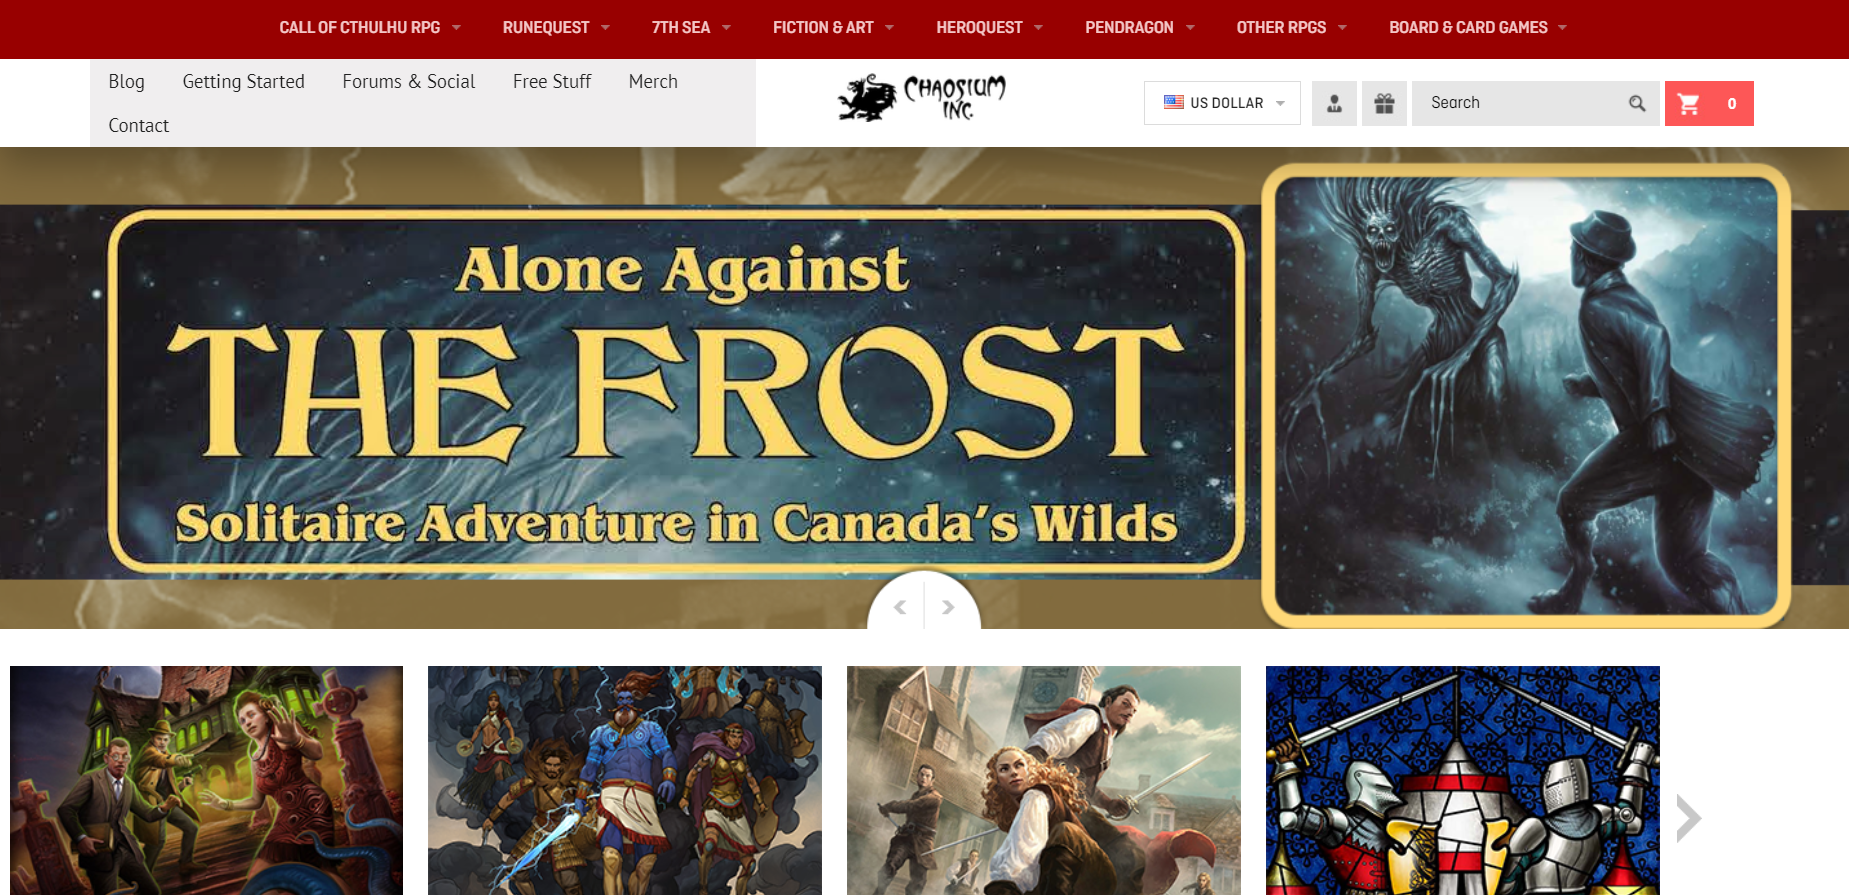
\includegraphics[width=1\textwidth]{{Zdjecia/ChaosiumInc.png}}
	\caption{Strona główna Chaosium Inc.}
\end{figure}

\subsection {Copernicus Corporation}

Strona jednego ze starszych polskich wydawnictw, mająca w swoim portfolio takie tytuły jak Warhammer, Dark Heresy czy Wiedźmin. Około dwóch lat temu przeszła gruntowną przemianę.

Odświeżona szata graficzna prezentuje się na prawdę dobrze - po stronie porusza się najlepiej ze wszystkich tutaj porównywanych. Szata graficzna czy czcionka są dobrane bardzo ostrożnie, przez co miejscami wypadają nijako. Brak multimediów.

Zamawianie produktów także nie stanowi jakiegokolwiek problemu. Dosyć istotną wadą jest brak możliwości wysyłki Pocztą Polską. W przypadku dużych miast większość osób i tak wybierze paczkomat, nie są to jednak jedyni klienci Copernicusa. 

Strona wydawnictwa Andrzeja Karlickiego wypada blado pod względem dodatków. Nie ma wszystkich oficjalnych, darmowych materiałów, trudno szukać kości, sakiewek czy innych ciekawych treści, które da się odnaleźć w internecie. 

\begin{figure}[H]
	\centering
	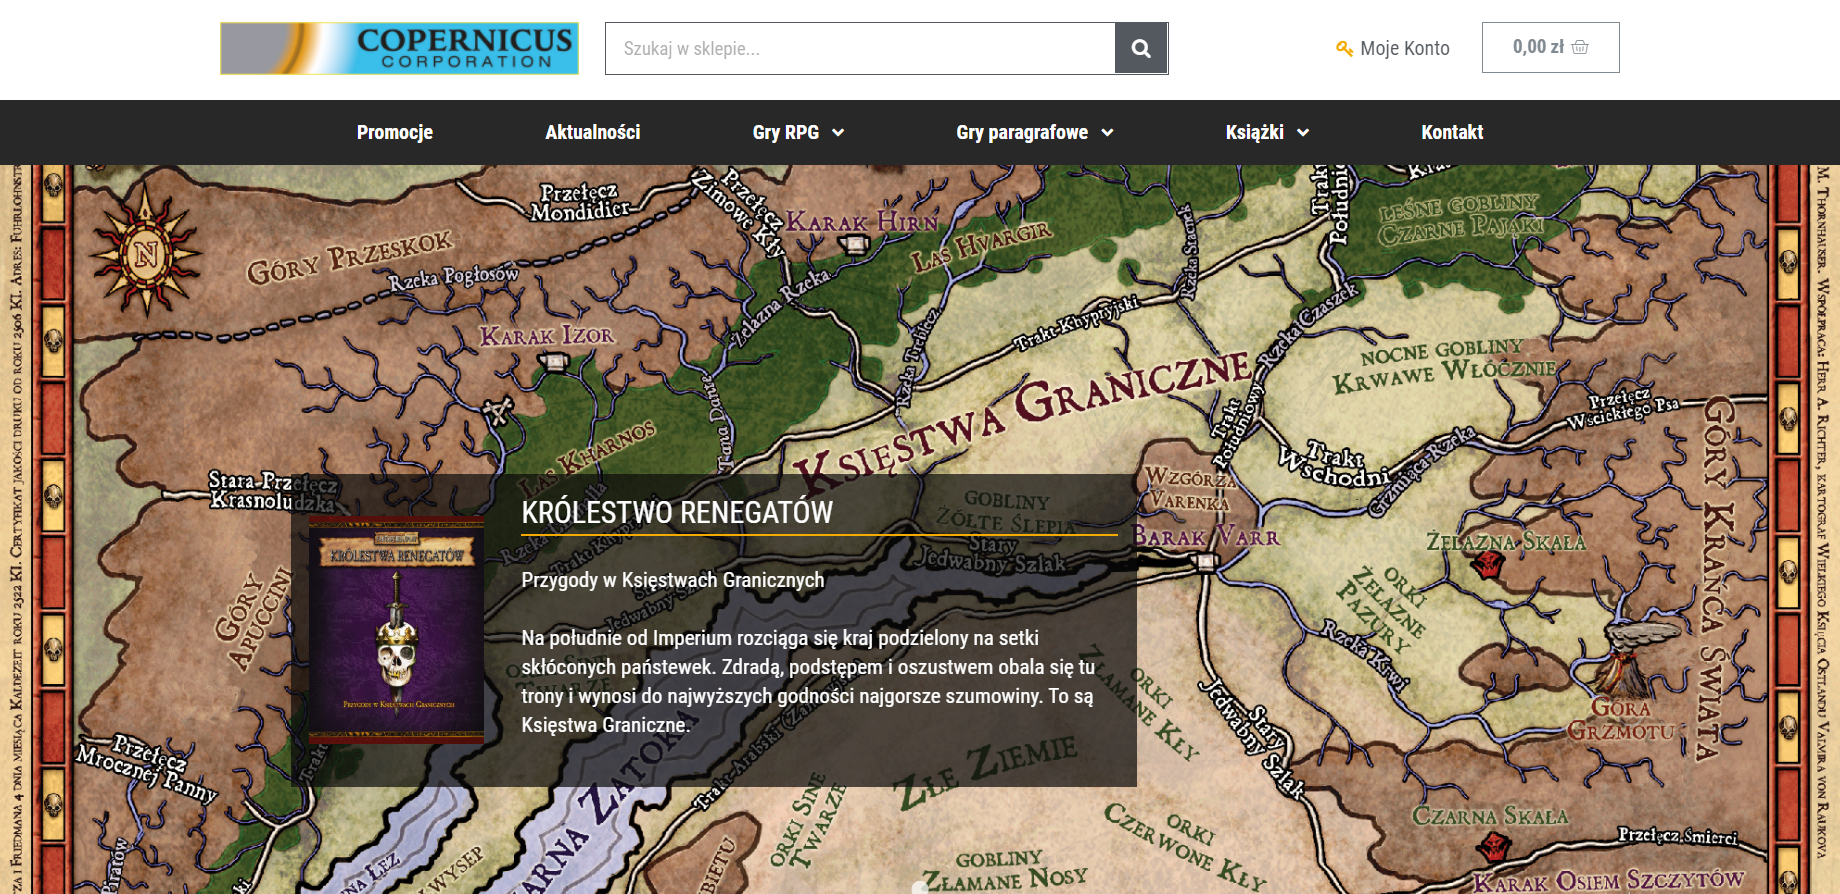
\includegraphics[width=1\textwidth]{{Zdjecia/Copernicus.png}}
	\caption{Strona główna Copernicus Corporation.}
\end{figure}

\subsection {Dungeons \& Dragons - Rebel}

Wydawnictwo Rebel wydając najnowszą edycję Dungeons \& Dragons zdecydowało się stworzyć specjalną stronę dla systemu, zamiast polegać tylko na własnym sklepie obecnym od lat. 

Strona wygląda rewelacyjnie. Wszystko dobrze się ze sobą komponuje, będąc przy okazji czytelnym. Układ strony sprawdziłby się trochę lepiej przy mniejszej liczbie treści. Doskonale wyważona liczba multimediów jest kolejną zaletą.

Część funkcjonalna to w dużej mierze ocena wielobranżowego sklepu Rebel, pozwalający zaopatrywać się w jednym miejscu fanom gier planszowych, karcianych, edukacyjnych jak i oczywiście gier fabularnych. Strona ta, będąc prostą i dającą dużo różnych możliwości, przeciętnie sprawdza się na urządzeniach mobilnych, zakładka kontaktowa także prezentuje się przeciętnie. 

Pod względem innych dodatków, strona nie wykorzystuje wszystkich możliwości jakie daje wydawca zza oceanu, nie zbierając tak wiele materiałów przydatnych dla doświadczonych graczy. Nie posiada FAQ, które pozwoliłyby użytkownikom na szybsze uzyskanie odpowiedzi na pytanie. Brak strony na Facebooku oraz newslettera sprawia, że gracze nie mogą być na bieżąco z ofertą wydawnictwa. Jest jednak jeszcze więcej plusów. Strona ta świetnie się sprawdzi dla graczy zaczynających zabawę z grami fabularnymi. Zebranie przeróżnych odnośników do stron czy kanałów transmitujących sesje Lochów i Smoków na żywo to strzał w dziesiątkę.  

\begin{figure}[H]
	\centering
	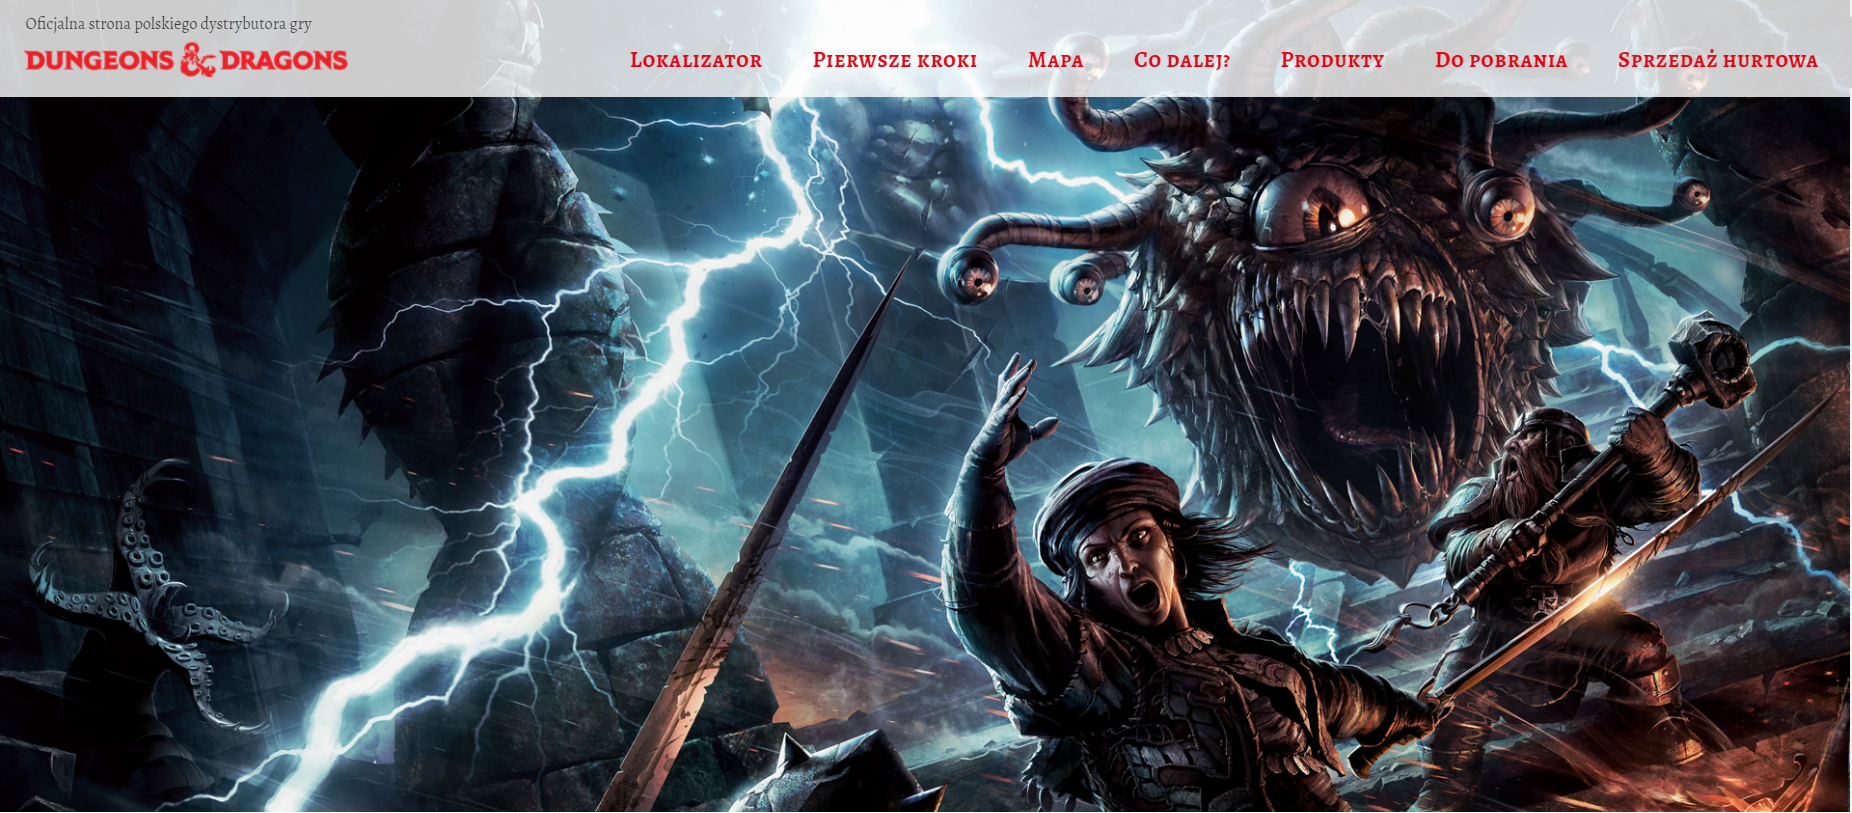
\includegraphics[width=1\textwidth]{{Zdjecia/DD.png}}
	\caption{Strona główna Dungeons \& Dragons wydawnictwa Rebel.}
\end{figure}

\subsection {Dungeons \& Dragons - Wizards of the Coast}

Najbardziej znany system fabularny na świecie posiada bardzo potężną stronę internetową, która pod względem dodatkowego wsparcia nie może się równać z żadną inną. Marka jest na tyle mocna na rynku, że D\&D to już nie tylko gry fabularne, ale i gry na komputer czy gry bitewne, które są zebrane w jednym miejscu. 

Wygląd strony przypomina omawianą wcześniej witrynę wydawnictwa Rebel. Szata graficzna jest przejrzysta oraz czytelna. Obecne multimedia doskonale wpasowują się w charakter strony. 

Jeśli chodzi o część funkcjonalną, to dostajemy pokaźną ilość odnośników do stron innych sprzedawców, dzięki którym zamówimy angielskie książki nawet do Polski, jest to jednak delikatne utrudnienie - bezpośrednio na witrynie nie jesteśmy w stanie nic kupić. (stąd po jednym punkcie w kategoriach zapłaty i dostawy). Panel kontaktowy jest rozbudowany i bogaty, a aplikacja mobilna świetnie się prezentuje.

Opis świata, mapa sklepów stacjonarnych, dodatki na komputer takie jak tapety czy aplikacje oraz streamy to tylko nieliczne z zalet. W przeciwieństwie do polskiej strony Dungeons \& Dragons, otrzymujemy link do Facebooka oraz FAQ. Jako jedyna strona z przez nas porównywanych nie posiada opinii o produkcie, co zmusza użytkownika do poszukiwania informacji poza omawianą przez nas witryną. 



\begin{figure}[H]
	\centering
	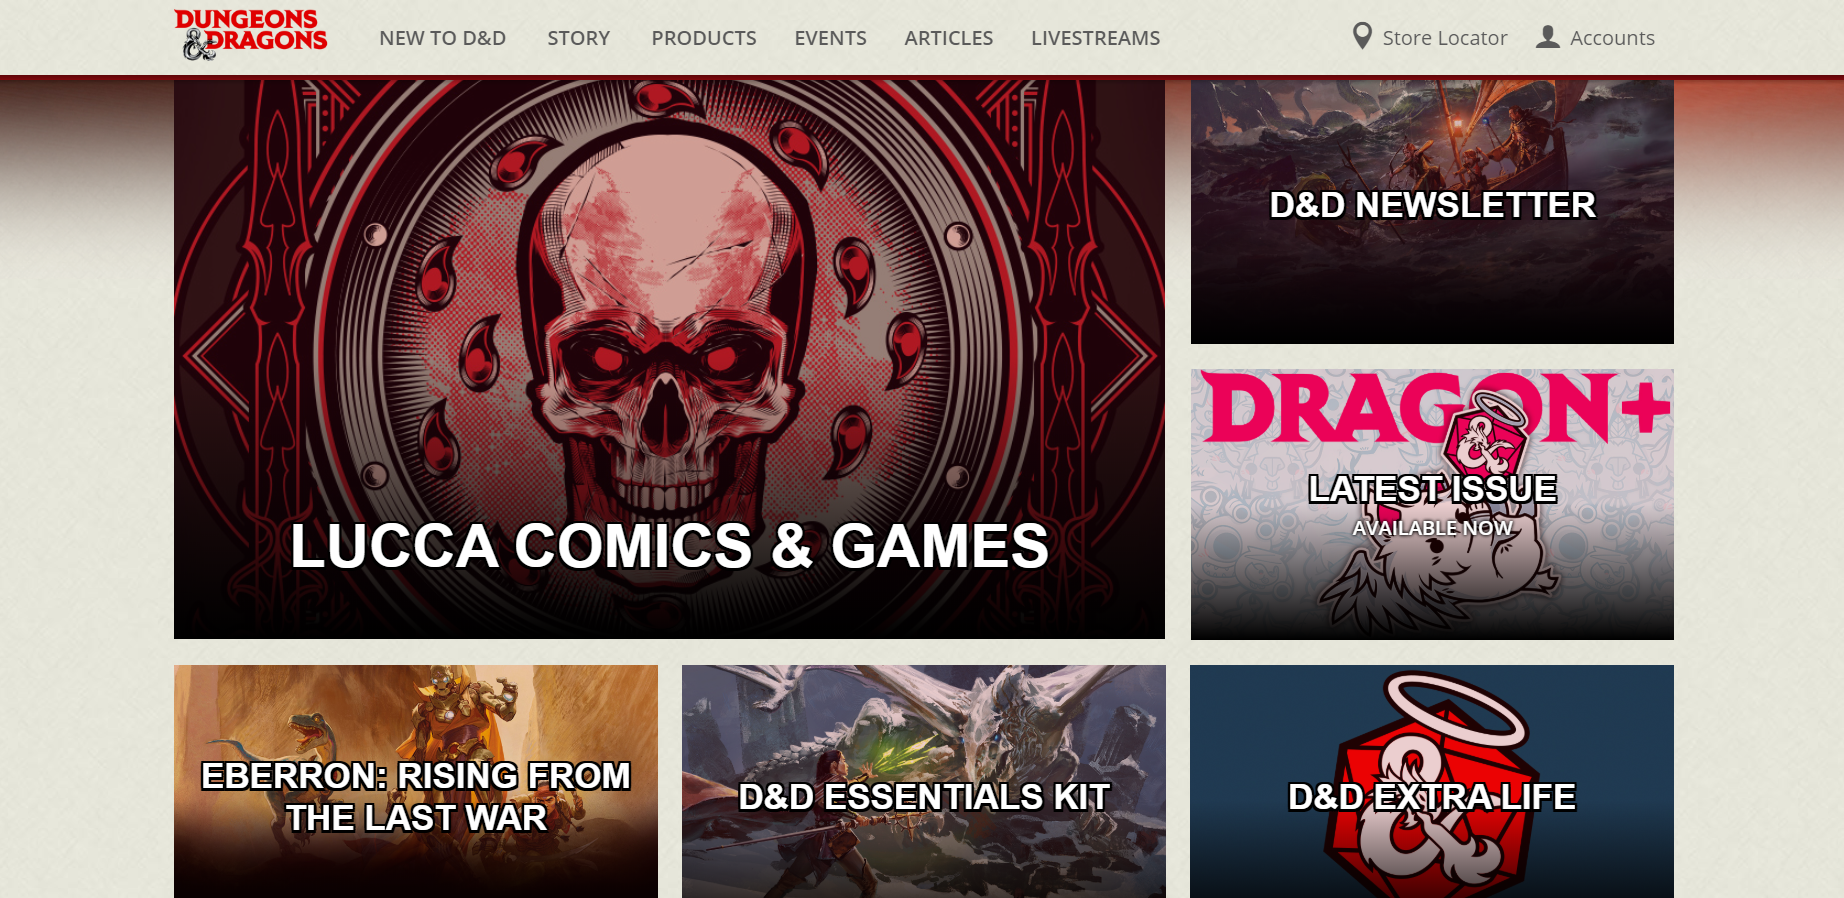
\includegraphics[width=1\textwidth]{{Zdjecia/DDEng.png}}
	\caption{Strona główna Dungeons \& Dragons wydawnictwa Wizards of the Coast.}
\end{figure}

\subsection {Hengal}

Nowe wydawnictwo, mające ledwie ponad rok, które utworzyło się po sukcesie zbiórki na serwisie wspieram.to, gdzie zebrali ponad 450\% wymaganej kwoty do wydania \textbf{Słowian} - gry fabularnej wzorującej się mitach słowiańskich. 

Sklep wydawnictwa już zdążył przejść przemianę, zdecydowanie wyprzedzając jakościowo część portalu skupiającą artykuły, zapowiedzi i materiały dodatkowe. Po pozostałej części witryny porusza się wyjątkowo ciężko, szata graficzna jest niespójna miedzy różnymi podstronami. Hengal został przez nas najsłabiej oceniony w części graficznej.

W części funkcjonalnej strona omawianego wydawnictwa otrzymała maksymalną liczbę punktów. Bogaty opis produktów, różne opcje zapłaty oraz zapewniony atrakcyjny panel kontaktowy uatrakcyjniają  witrynę. Wersja mobilna również wygląda przejrzyście oraz czytelnie. 

Wyraźnie widoczny link do strony na Facebooku zaliczamy do zalet. Hengal zadbał także o FAQ oraz neswlettera. Wydawnictwo oferuje promocje na swoje produkty, jednakże liczba ich reklama jest przytłaczająca. Z drugiej strony, ilość materiałów dodatkowych jest pozytywnie oszałamiająca - jest to tym większym plusem, że system jest zdecydowanie mniej popularny od wcześniej tu porównywanych RPGów. Oferowanie bogatej ofert materiałów dodatkowych wpłynęło na zwycięstwo sklepu wydawnictwa Hengal w kategorii inne. 

\begin{figure}[H]
	\centering
	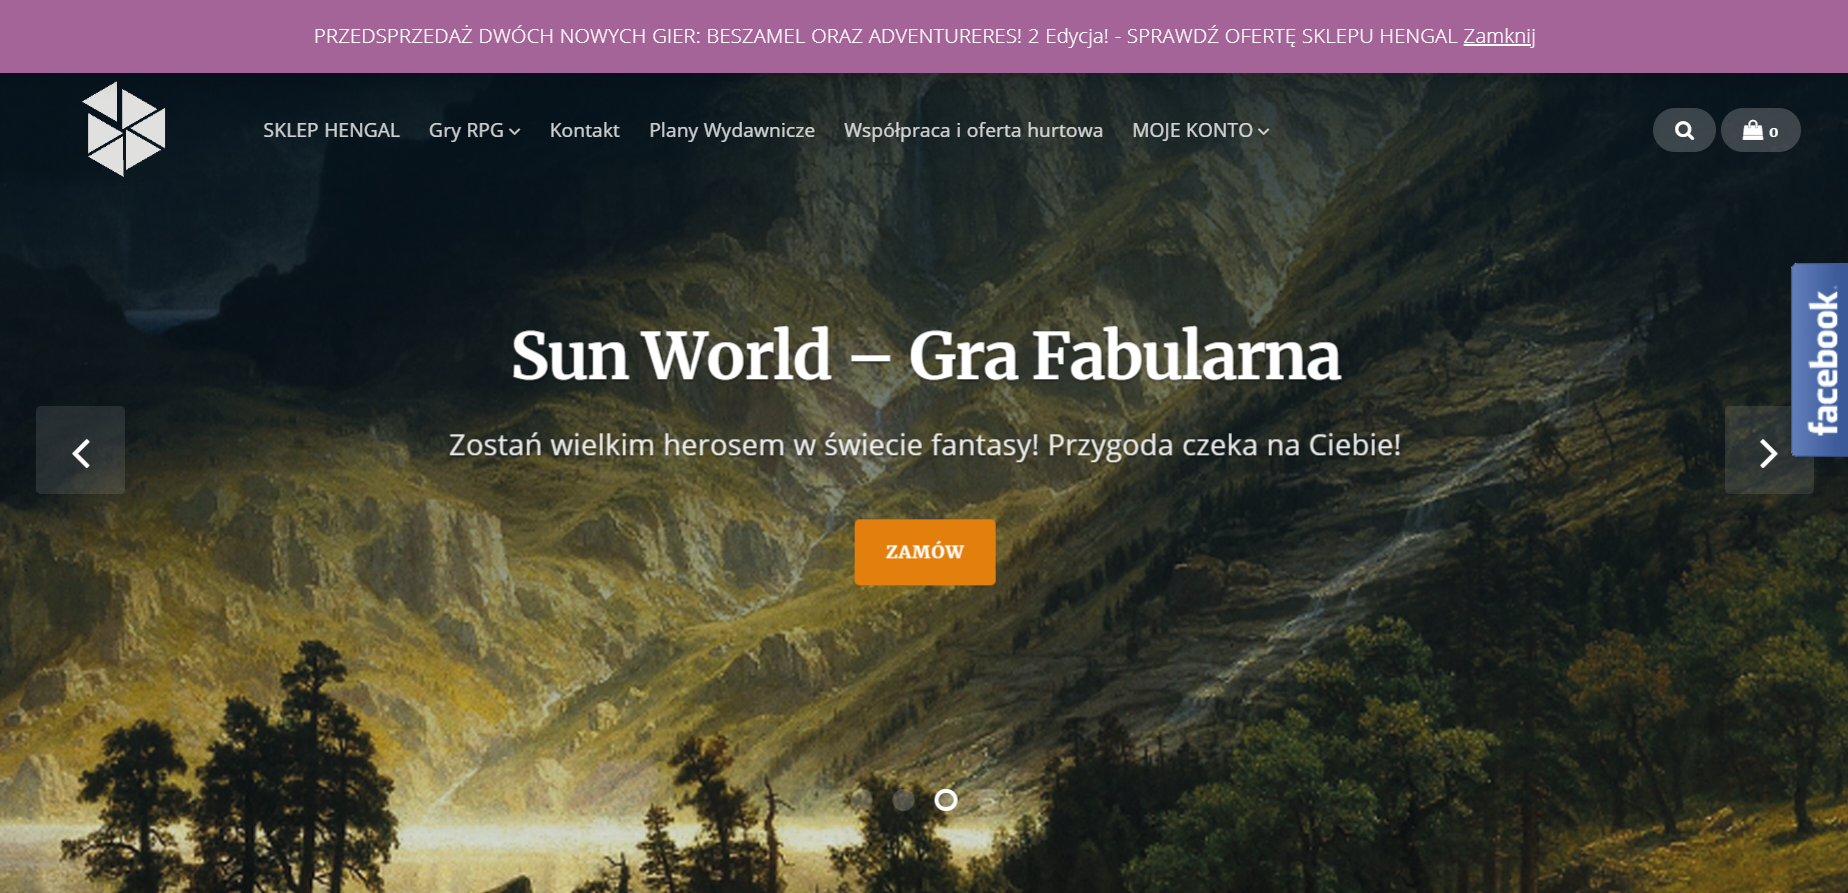
\includegraphics[width=1\textwidth]{{Zdjecia/Hengal.png}}
	\caption{Strona główna Dungeons \& Dragons wydawnictwa Wizards of the Coast.}
\end{figure}

\newpage

\section {Punktacja}

\begin{tabular}{|l|c||c|c|c|c|c|}
	\hline
	
	\multicolumn{1}{|c}{\textbf{Kryterium}} & \multicolumn{1}{|c||}{\textbf{Pkt}} & \multicolumn{1}{c}{\textbf{Chaosium}} & \multicolumn{1}{|c}{\textbf{CopCorp}} & \multicolumn{1}{|c}{\textbf{D\&D PL}} &\multicolumn{1}{|c}{\textbf{D\&D EN}} &\multicolumn{1}{|c|}{\textbf{Hengal}}\\
	\hline \hline
	
	\multicolumn{7}{|c|}{\textbf{Kryterium graficzne (11 punktów)}} \\
	\hline
	Szata graficzna & 3 & 2 & 2 & 3 & 3 & 2 \\
	\hline
	Układ strony & 3 & 2 & 3 & 2 & 2 & 1 \\ 
	\hline
	Czcionka & 3 & 1 & 2 & 3 & 2 & 1 \\ 
	\hline
	Multimedia & 2 & 1 & 1 & 2 & 2 & 1 \\ 
	\hline \hline
	SUMA & 11 & 6 & 9 & 10 & 9 & 5 \\ 
	\hline \hline

	\multicolumn{7}{|c|}{\textbf{Kryterium funkcjonalne (13 punktów)}} \\
	\hline
	Opis produktów & 3 & 3 & 3 & 3 & 3 & 3 \\ 
	\hline
	Opcje zapłaty & 2 & 2 & 2 & 2 & 1 & 2 \\ 
	\hline
	Opcje dostawy & 2 & 2 & 1 & 2 & 1 & 2 \\ 
	\hline
	Bezpieczeństwo & 1 & 1 & 1 & 1 & 1 & 1 \\ 
	\hline
	Konstrukcja menu & 1 & 1 & 1 & 1 & 1 & 1 \\ 
	\hline
	Kontakt & 2 & 2 & 2 & 1 & 2 & 2 \\ 
	\hline
	Wersja mobilna & 2 & 2 & 2 & 1 & 2 & 2 \\ 
	\hline \hline
	SUMA & 13 & 13 & 12 & 11 & 11 & 13 \\ 
	\hline \hline
	
	\multicolumn{7}{|c|}{\textbf{Inne (11 punktów)}} \\
	\hline
	Dodatkowe materiały & 3 & 2 & 2 & 1 & 3 & 3 \\ 
	\hline
	Opinie o produkcie & 1 & 1 & 1 & 1 & 0 & 1 \\ 
	\hline
	Dodatkowa oferta & 1 & 0 & 0 & 1 & 1 & 1 \\ 
	\hline
	Newsletter & 1 & 1 & 1 & 0 & 0 & 1 \\ 
	\hline
	Promocje & 1 & 0 & 1 & 1 & 0 & 1 \\ 
	\hline
	Link do Facebooka & 1 & 1 & 1 & 0 & 1 & 1 \\ 
	\hline
	FAQ & 1 & 0 & 1 & 0 & 1 & 1 \\ 
	\hline
	Inne & 2 & 1 & 0 & 2 & 2 & 0 \\ 
	\hline \hline
	SUMA & 11 & 6 & 7 & 7 & 8 & 9 \\ 
	\hline \hline
	
	\multicolumn{7}{|c|}{\textbf{Całość (35 punktów)}} \\
	\hline
	SUMA & 35 & 25 & 27 & 28 & 28 & 27 \\ 
	\hline
	
\end{tabular}


\section {Wnioski}
\begin{itemize}
	\item Porównywane przez nas strony wedle przyjętych przez nas kryteriów prezentują podobny poziom,
	\item Na wysokim poziomie stoi część funkcjonalna, dzięki czemu bez problemu możemy zakupić interesujące nas podręczniki,
	\item Wydawnictwa nie zbierają wielu porządnie wykonanych, fanowskich materiałów.
	\item Szata graficzna na stronach wydawców gier fabularnych nie prezentuje poziomu, do którego przyzwyczają nas globalne marki.
\end{itemize} 

\end{document}